Um Informationen bzw. Bits zu manipulieren werden Schaltungen ben\"otigt welche Gatter beinhalten, dies gilt f\"ur klassische Rechner und Quantencomputer. Um in der Digitaltechnik die Funktionsweise von Gattern darzustellen werden gerne Wahrheitstabellen genutzt (rechte Spalte Tabelle \ref{table:Qubit-Gatter}). Bekannte Gatter-Typen aus der Digitaltechnik, wie der Negation oder dem Exklusiv-ODER k\"onnen auch in der Welt der Quantencomputer abgebildet werden. Jedoch ist der Aufbau dieser Gatter etwas gew\"ohnungsbed\"urfdig, denn die Realisierung eines auf $n$ Qubits operierenden Gatters erfolgt durch eine unit\"are $2^{n}\times 2^{n}$-Matrix. Die Anwendung eines Gatters auf einen Zustandvektor entspricht mathematisch also einer unit\"aren Transformation auf den Zustandsvektor und f\"uhrt eine Rotation auf der Bloch-Kugel aus. Dies geschieht durch die Bildung des Skalarprodukts \"uber der unit\"aren Matrix und dem Zustandvektor. \\ \\
Eine Matrix wird als unit\"ar bezeichnet, wenn das Produkt aus dieser Matrix und dessen adjungierte Matrix eine Einheitsmatrix bildet.
\begin{equation}
  I = A^{\dagger} A
\end{equation}
Die Adjungierte Matrix wird gebildet, indem alle Eintr\"age in dieser Matrix komplex konjungiert und transponiert werden.
\begin{equation}
  A^{\dagger} = A^{*T}
\end{equation}

Somit sind alle Quantengatter unit\"are Matrizen, genau wie die drei aus der Quantenmechnik bekannten Paulimatrizen $X, Y$ und $Z$ Tabelle \ref{table:Qubit-Gatter}. Diese f\"uhren eine Rotation von $\pi$ um die $x, y$ und $z$-Achse auf der Bloch-Kugel durch. Das Hadamard-Gatter $H$ erm\"oglicht einen Abweichung der Basiszust\"ande $|0\rangle$ und $|1\rangle$ und erzeugt somit Superpositionen dieser \cite{Qiskit-Textbook}.
Dies w\"aren die Zustandvektoren $|+\rangle$ und $|-\rangle$, welche auch auf der Bloch-Kugel in Abbildung \ref{fig:Bloch-Kugel} zu erkennen sind. \\ \\
Zwei parametrisierte Gatter, das $P$-Gatter (Phasen-Gatter) und $U$-Gatter die nicht in Tabelle \ref{table:Qubit-Gatter} aufgef\"uhrt sind, erlauben die Spezifizierung von s\"amtlichen Gattern bzw. unedlich vielen Gattern.
\begin{equation}
\begin{aligned}
P(\phi) &= \begin{bmatrix}1 & 0 \\ 0 & e^{i\phi} \end{bmatrix} &&\qquad \phi \in \mathbf{R}\\[1em]
U(\theta, \phi, \lambda) &= \begin{bmatrix} \cos\left(\frac{\theta}{2}\right) & -e^{i\lambda}sin\left(\frac{\theta}{2}\right) \\
e^{i\phi}sin\left(\frac{\theta}{2}\right) & e^{i(\phi+\lambda)}sin\left(\frac{\theta}{2}\right)
\end{bmatrix} &&\qquad \theta, \phi, \lambda \in \mathbf{R}
\end{aligned}
\end{equation}

\vspace{1.2cm}
%%%%%%%%%%%%%%%%%%%%%%%Table%%%%%%%%%%%%%%%%%%%%%%%%%%%%%%%%

\begin{table}[h] 
\begin{tabular}{@{\hspace{1cm}}c@{\hspace{1cm}} | @{\hspace{1cm}}c@{\hspace{1cm}} | @{\hspace{1cm}}c@{\hspace{1cm}}}
\hline 
Matrix & Schaltungssymbol & Wahrheitstabelle \\
\hline & \\
$X = \begin{bmatrix} 0 & 1 \\ 1 & 0 \end{bmatrix}$ &
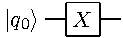
\includegraphics[width=0.2\textwidth]{figures/pauli_x.pdf} &
\begin{tabular}{|c||c||c|}
\hline
Fall & $|q\rangle$ & $X|q\rangle$ \\
\hline \hline 
1 & $|0\rangle$ & $|1\rangle$ \\
2 & $|1\rangle$ & $|0\rangle$ \\
\hline
\end{tabular} \\&\\

%%%%%%%%%%%%%%%%%%%%%%%%%%%%%%%%%%%%%%%%%%%%%%%%%%%%%%%%%%%%%%

$Y = \begin{bmatrix} 0 & -i \\ i & 0 \end{bmatrix}$ &
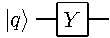
\includegraphics[width=0.2\textwidth]{figures/pauli_y.pdf} &
\begin{tabular}{|c||c||c|}
\hline
Fall & $|q\rangle$ & $Y|q\rangle$ \\
\hline \hline 
1 & $|0\rangle$ & $i|1\rangle$ \\
2 & $|1\rangle$ & $-i|0\rangle$ \\
\hline
\end{tabular} \\&\\

%%%%%%%%%%%%%%%%%%%%%%%%%%%%%%%%%%%%%%%%%%%%%%%%%%%%%%%%%%%%%%

$Z = \begin{bmatrix} 1 & 0 \\ 0 & -1 \end{bmatrix}$ &
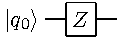
\includegraphics[width=0.2\textwidth]{figures/pauli_z.pdf} &
\begin{tabular}{|c||c||c|}
\hline
Fall & $|q\rangle$ & $Z|q\rangle$ \\
\hline \hline 
1 & $|0\rangle$ & $|0\rangle$ \\
2 & $|1\rangle$ & $-|1\rangle$ \\
\hline
\end{tabular} \\&\\

%%%%%%%%%%%%%%%%%%%%%%%%%%%%%%%%%%%%%%%%%%%%%%%%%%%%%%%%%%%%%%

$H = \frac{1}{\sqrt{2}} \begin{bmatrix} 1 & 1 \\ 1 & -1 \end{bmatrix}$ &
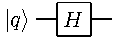
\includegraphics[width=0.2\textwidth]{figures/hadamard.pdf} &
\begin{tabular}{|c||c||c|}
\hline
Fall & $|q\rangle$ & $H|q\rangle$ \\
\hline \hline 
1 & $|0\rangle$ & $\frac{|0\rangle+|0\rangle}{\sqrt{2}}$ \\
2 & $|1\rangle$ & $\frac{|0\rangle-|1\rangle}{\sqrt{2}}$ \\
\hline
\end{tabular} \\&\\

%%%%%%%%%%%%%%%%%%%%%%%%%%%%%%%%%%%%%%%%%%%%%%%%%%%%%%%%%%%%%%

$S = \begin{bmatrix} 1 & 0 \\ 0 & i \end{bmatrix}$ &
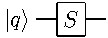
\includegraphics[width=0.2\textwidth]{figures/phase.pdf} &
\begin{tabular}{|c||c||c|}
\hline
Fall & $|q\rangle$ & $S|q\rangle$ \\
\hline \hline 
1 & $|0\rangle$ & $|0\rangle$ \\
2 & $|1\rangle$ & $i|1\rangle$ \\
\hline
\end{tabular} \\&\\

%%%%%%%%%%%%%%%%%%%%%%%%%%%%%%%%%%%%%%%%%%%%%%%%%%%%%%%%%%%%%%

$T = \begin{bmatrix} 1 & 0 \\ 0 & e^{i\frac{\pi}{4}} \end{bmatrix}$ &
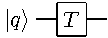
\includegraphics[width=0.2\textwidth]{figures/t_dagger.pdf} &
\begin{tabular}{|c||c||c|}
\hline
Fall & $|q\rangle$ & $T|q\rangle$ \\
\hline \hline 
1 & $|0\rangle$ & $|0\rangle$ \\
2 & $|1\rangle$ & $e^{i\frac{\pi}{4}} |1\rangle$ \\
\hline
\end{tabular} \\&\\
\hline
\end{tabular}
\caption{Grundlegende 1-Qubit Gatter}
\label{table:Qubit-Gatter}
\end{table}
\clearpage

Aus dem $P$-Gatter lassen sich die Gatter $Z, S$ und $T$ konstruieren. \ref{eqn:konstruktion} zeigt die Spezifizierung der $S$- und $T$-Gatter durch das Phasengatter.
\begin{equation}\label{eqn:konstruktion}
P\left(\phi=\frac{\pi}{2}\right) = S \qquad P(\phi=\pi) = Z .
\end{equation}

Das $U$-Gatter erm\"oglicht die Spezifizierung jeglicher Gatter, z.B. kann das Hadamard-Gatter folgenderma\ss en durch das $U$-Gatter spezifiziert werden
\begin{equation}
U\left(\theta= \frac{\pi}{2}, \phi=0, \lambda=\pi\right) = H .
\end{equation}
Somit kann es eine gro\ss e Menge an n\"utzlichen Gattern geben, die auf 1-Qubit operieren.
